\chapter{Implementation of Direct GPU-FPGA Communication}
\label{section:implementation}

\section{Environment}

As simulation environment I am using V-REP 3.4.0\cite{Rohmer2013}

SNN controllers are implemented using NEST simulator 2.14.0\cite{Peyser2017}

The simulation and the python controller communicate over ROS kinetic\cite{}



\begin{lstlisting}[label=listing:example_code, caption=example]
code = example
\end{lstlisting}

\section{Setup}

\begin{figure}
	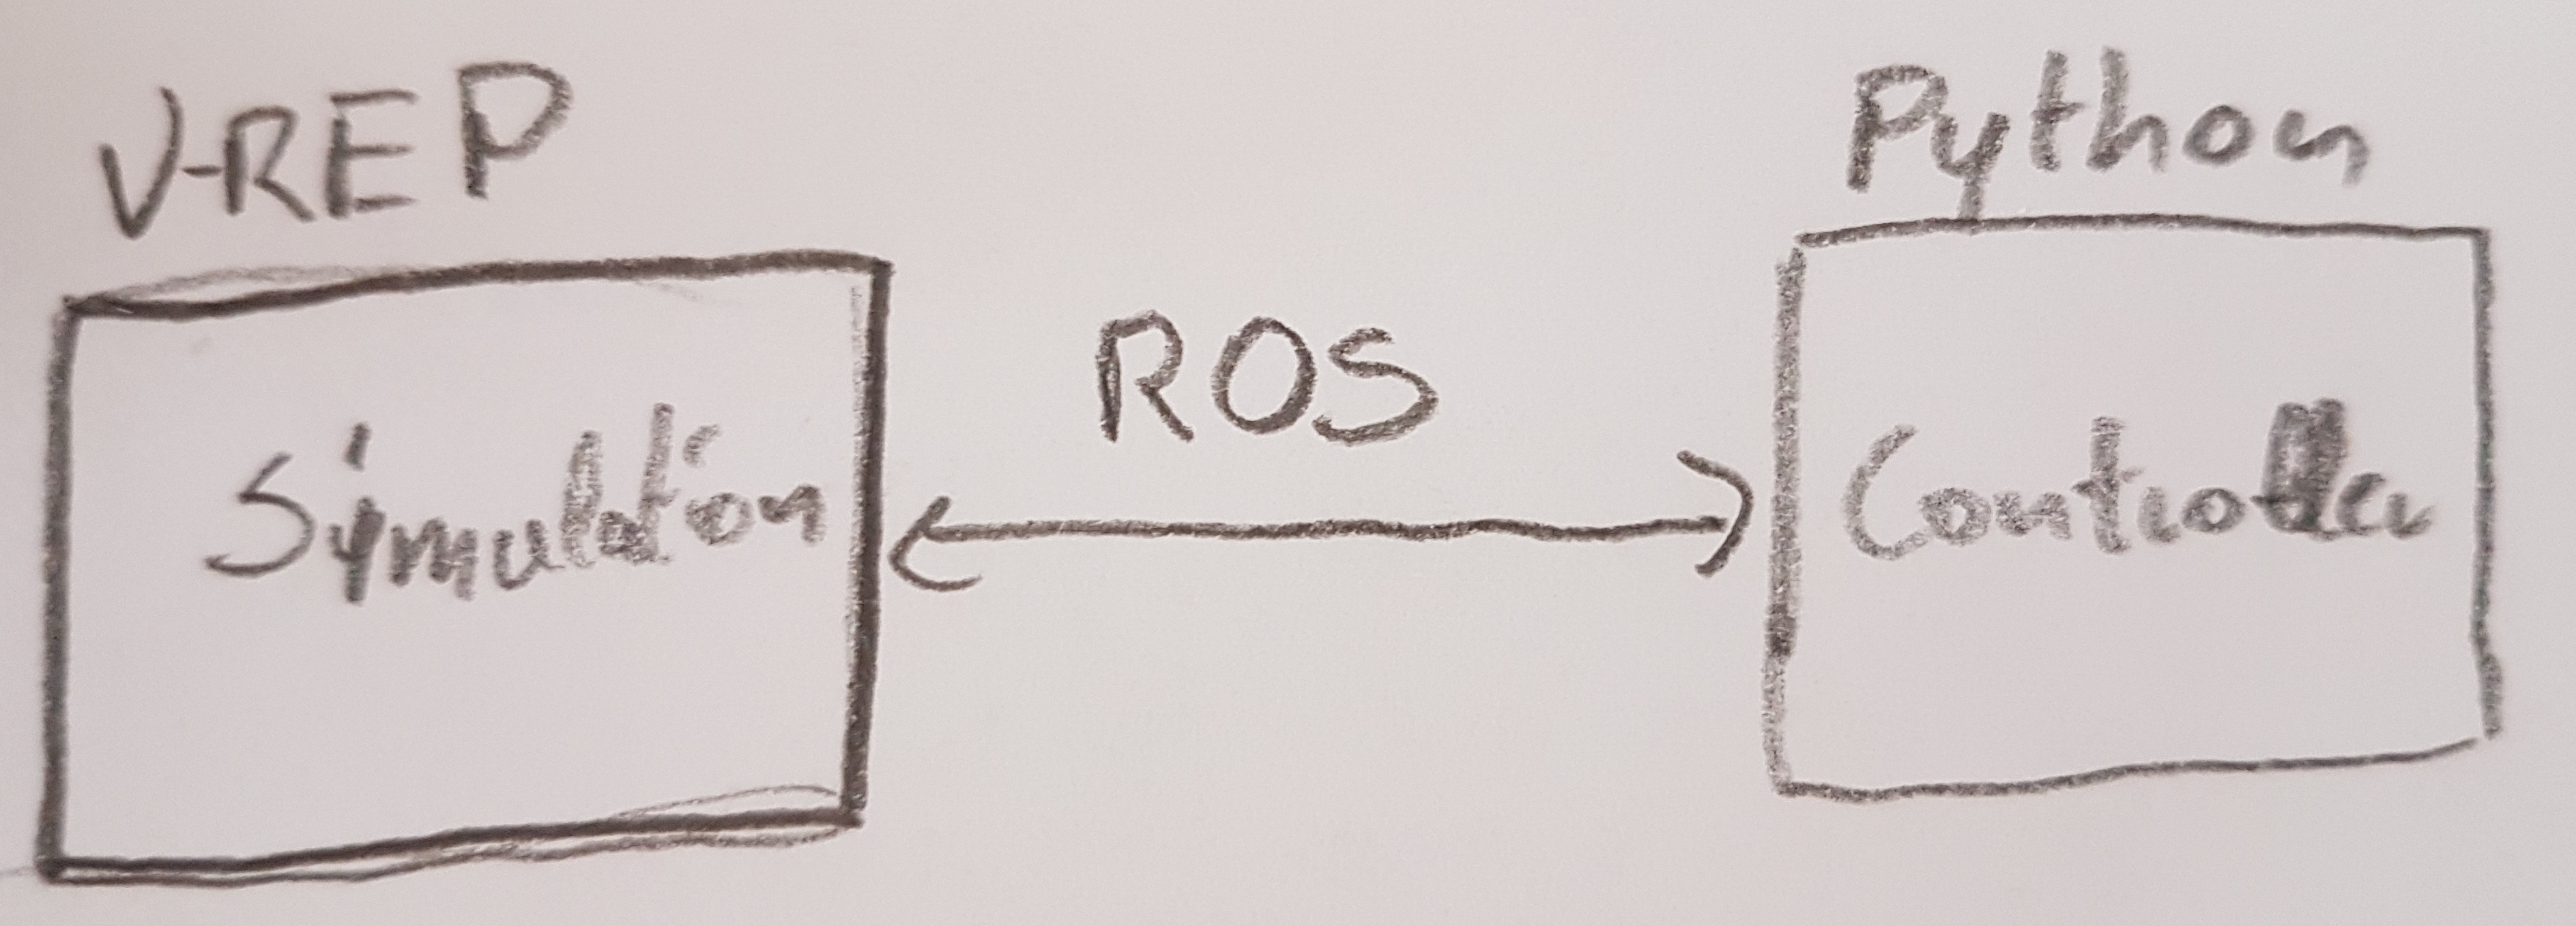
\includegraphics[width=\linewidth]{images/setup.jpg}
	\caption{The two main components and the communication channel}
	\label{fig:setup}
\end{figure}


This section gives a high overview of the experiment. In figure \ref{fig:setup} you can see that there are two main components. First we have the simulation made with V-Rep witch contains the snake like robot and the environment. The environment is made out of a target ball the snake will learn to follow and obstacles in the form of walls. The snake moves according to the movement model from section \ref{section:model}. The second important component is the python controller that will learn to manoeuvre the snake through the environment successfully. The structure of the controller is described in detail in the following section. It contains SNN that will solve a target following and an obstacle avoidance task. The SNN are implemented using the NEST simulator. Both components communicate with each other using ROS. They are both ROS nodes and can exchange messages over the ROS Topic messaging protocol.


\section{Target Following Controller}

The goal of the target following controller is it to successfully follow a target trough the environment. In our simulation the target is represented by a warm ball that can be seen by the infrared camera on the head of the snake.